\section{Implementation}
\label{section:implementation}
\subsection{Mobile Player}
In this section the mobile player \gls{prefab} will be discussed. 
\gls{see} is supported on multiple platforms and with each platform having different requirements each platform needs to be divided.
Therefore, each platform gets its own player \gls{prefab}.
The mobile player prefab for the \gls{android} version of \gls{see} can be seen in figure \ref{fig:prefab}.

\begin{figure}[htb]
    \centering
    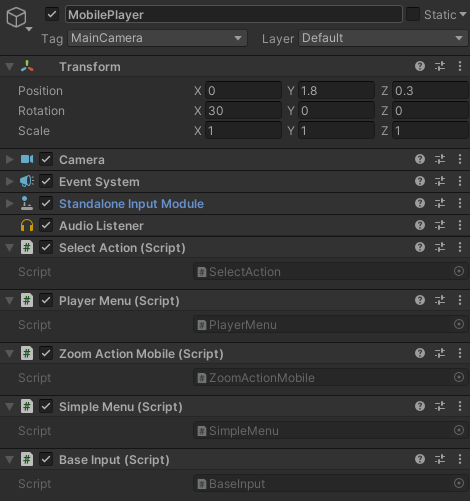
\includegraphics[width=0.8\textwidth]{Implementation/img/mobile_player.png}
    \caption{The mobile player \gls{prefab}}\label{fig:prefab}
\end{figure}

The \gls{prefab} consists of the basic parts provided by \gls{unity} \textit{Camera}, \textit{Event System}, \textit{Standalone Input Module} and \textit{Audio Listener}.
In addition to that the following custom scripts were added.
There is the \textit{SelectAction} and the \textit{ZoomActionMobile} script, which will both be discussed in section \ref{sec:player_actions}, and then there is the \textit{PLayerMenu} script, which creates the right menu based on the player type.
In this case the player type will be \enquote{mobile player} and the menu created (here \textit{SimpleMenu}) will be discussed in section \ref{sec:menu}.

\subsection{Player Movement}
After having creating a player, the player also has to be able to move.
Therefore, the \textit{MobilePlayerMovement} script got added.
The script handles the input by the joysticks seen in figure \ref{fig:joystick}.
To fulfill [R2.1] the player will be moved by using the left joystick and the player's perspective will be handled by the right joystick.


\begin{figure}[htb]
    \centering
    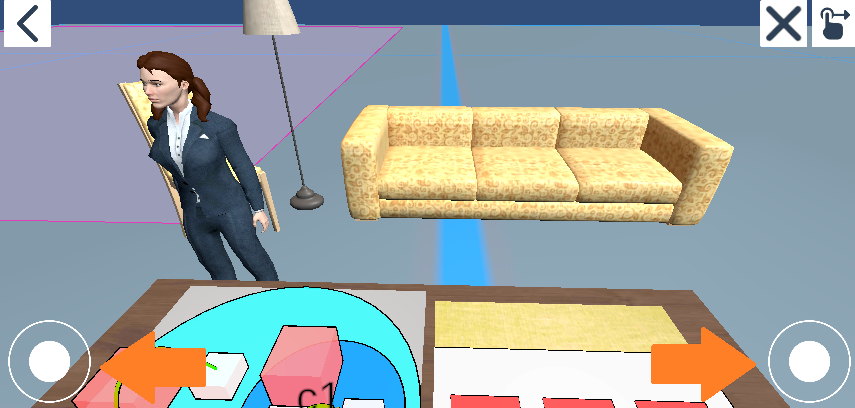
\includegraphics[width=1\textwidth]{Implementation/img/joysticks.png}
    \caption{The joysticks are for moving in the virtual room. The left joystick is for moving the player and the right one is for moving the player's perspective.}\label{fig:joystick}
\end{figure}

\subsection{Mobile Menu}
\label{sec:menu}
\begin{figure}[htb]
    \centering
    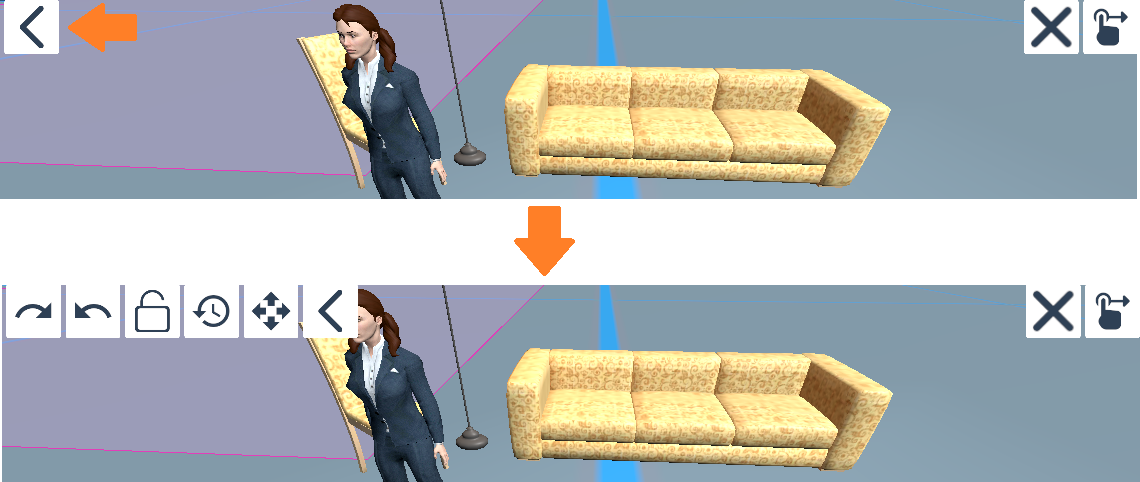
\includegraphics[width=1\textwidth]{Implementation/img/quickmenu.png}
    \caption{The \textit{quickmenu} on the left top side of the mobile device. Pressing the button with an orange marked arrow will expand the menu.}\label{fig:quickmenu}
\end{figure}

\begin{figure}[htb]
    \centering
    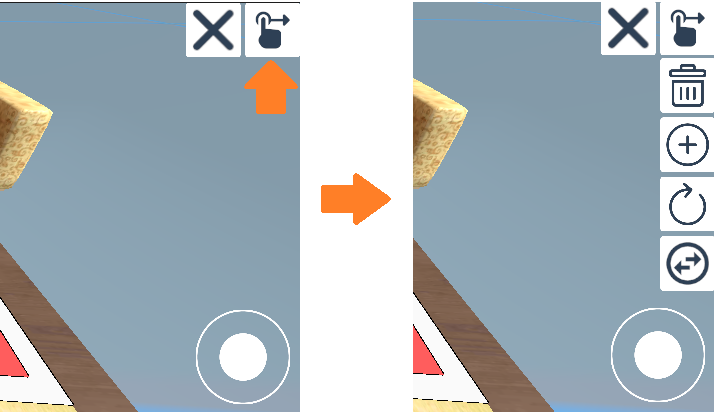
\includegraphics[width=1\textwidth]{Implementation/img/menu.png}
    \caption{The player interaction menu on the right top side of the mobile device. The button on the top right side indicate the active interaction mode. Pressing the same button also expands the menu.}\label{fig:menu}
\end{figure}

\subsection{Player Actions}
\label{sec:player_actions}